%%%%%%%%%%%%%%%%%%%%%%%%%%%%%%%%%%%%%%%%%%%%%%%%%%%%%%%%%%%%%%%%%%%%%%%%%%%%%%%%%%%%%%%%%%%%%%%%%%%
%%%%%%%%%%%%%%%%%%%%%%%%%%%%%%%%%%%%%%%%%%%%%%%%%%%%%%%%%%%%%%%%%%%%%%%%%%%%%%%%%%%%%%%%%%%%%%%%%%%
\chapter{Resultados}

En cada canal que conforma el PSG (EEG, EOG y EMG), 
cada una de las \'epocas consideradas fue clasificada como 
''Posiblemente Estacionaria'' (PE) si no pudo ser rechazado la hip\'otesis de 
estacionariedad usando el test PSR ($\alpha = 0.05$), mientras que 
%el rechazo de esta misma 
%hip\'otesis es argumento ''suficiente'' para afirmar que el segmento de registro en cuenti\'on
%puede ser clasificado omo no.estacionario.
fue clasificado como ''No-estacionaria'' en caso contrario. Variar el valor cr\'itico
para la clasificaci\'on (siempre menor a 0.05) no pareci\'o generar diferencias significativas.
%La cantidad de \'epocas que no fueron para las cuales no es posible rechazar la hip\'otesis de
%estacionariedad ($\alpha=0.05$)
%clasificadas como ''Posiblemente Estacionarias'' (PE). 
La cantidad de \'epocas PE en cada individuo 
%con respecto a la cantidad total de \'epocas
durante el sue\~no MOR y no-MOR
muestra en las tablas \ref{total_gpos_mor}, \ref{total_gpos_nmor} y
\ref{total_gpos_total}; debido a que entre los sujetos hubo una gran variabilidad entre el tiempo 
que permanecieron en sue\~no MOR, se sugiri\'o comparar no el total de \'epocas PE sino
la proporci\'on --con respecto a la duraci\'on, medida en \'epocas-- de estas etapas, 
mustr\'andose estos resultados en las tablas \ref{gpos_mor}, \ref{gpos_nmor} y
\ref{gpos_total}. En estas \'ultimas tablas, se han calculado promedios y desviaciones
est\'andar muestrales entre los dos grupos que son comparados.


\begin{SidewaysFigure}
\centering
\begin{tabular}{c||ccccc||cccc||ccc}
&VCR&MJH&JAE&GHA&MFGR&CLO&RLO&RRU&JGZ&FGH&MGG&EMT \\
\hline
C3&**& &*&**& & &**&*& & & &  \\
C4&*& &***&*& & &***& & & &*&  \\
CZ&***& & & & & & & & & &***&  \\
F3&**& & &**& & &***& & & &*&** \\
F4& & & &*& & &***& & & &***&  \\
F7&*& &***&***& & & &*& & &***&*** \\
F8&**& & &**& & &*&*& & &***&  \\
FP1&***& & &*&*& & &*& & &***&  \\
FP2&***& & &*& & & & & & &***&  \\
FZ& & & &***& & &***&*& & &*&  \\
O1&*& & &***& & & & & &*& &  \\
O2& & &*&***& & &***& & & &***& \\ 
P3&*& &*&***& & &**& & & &*&  \\
P4&***& &***&*& & & & & &*&***&  \\
PZ&**& &***&*& & & &*& & &***&  \\
T3& & &**& & & &***& & & & &** \\
T4& & & &*& & &***& & & &*&  \\
T5&*& & &***& & &***& & & & &  \\
T6& & &*& & & & & & & &***&  \\
LOG&***& &***&***&**&***&**&***&*& &***&  \\
ROG&***& &***&***&*&*&***&*&*& &***&  \\
EMG& & & & & &***& &*& & & &  \\
\hline
General& & & & & &***& &*& & & & 
\end{tabular}
\caption{Diferencias significativas para la comparaci\'on entre la proporci\'on
de \'epocas PE en sue\~no MOR (fase R) y no-MOR (fases W y N).
Los asteriscos representan el pvalor con el cual se rechaza la hip\'otesis de
que las diferencias son significativas: *=0.05 , **=0.01 , ***=0.005}
\label{comparacion_mor_vs_total}
\end{SidewaysFigure}

Como un primer an\'alisis, para cada sujeto y en cada canal 
se compar\'o la proporci\'on de \'epocas PE en sue\~no MOR contra el registro completo;
el fin de ello es verificar si el sue\~no MOR --entendido como muestra no-aleatoria
del sue\~no-- tiene propiedades similares o no, y si \'esta similaridad pudiera estar
relacionada con el PDC del paciente. 
Las comparaciones se llevaron a cabo usando la prueba $\chi^{2}$ para 
proporciones\footnote{Implementada en R como la funci\'on \texttt{prop.test()}},
los resultados se muestran en la tabla \ref{comparacion_mor_vs_total}.
Se encontr\'o que no hay una relaci\'on clara entre el estado de salud del sujeto y
la aparici\'on de diferencias significativas entre estas proporciones, se hallaron
consistentemente diferencias en los canales LOG y ROG --que pueden explicarse como la actividad
ocular caracter\'istica del sue\~no MOR.
%; en la secci\'on
%de discusi\'on se mencionan algunos datos que se ''recuperaron'' de este an\'alisis.


Posteriormente se procedi\'o a comparar, por cada canal, si la proporci\'on de \'epocas PE
presenta diferencias significativas entre los grupos. Esta comparaci\'on se realiz\'o tomando
en cuenta las \'epocas de sue\~no MOR, de sue\~no no-MOR, y el registro completo 
--ver, respectivamente, tablas \ref{gpos_mor}, \ref{gpos_nmor}, \ref{gpos_total}.
Para una mejor visualizaci\'on de estos, se han graficado
% que representan
%las proporciones respectivas de cada sujeto --para ambos grupos.
en la figura \ref{comparacion_graf}
los datos de las tablas \ref{gpos_mor}, \ref{gpos_nmor} y
\ref{gpos_total}.

\begin{figure}
\centering
\subfloat[Comparaci\'on entre \'epocas MOR (fase R)]{
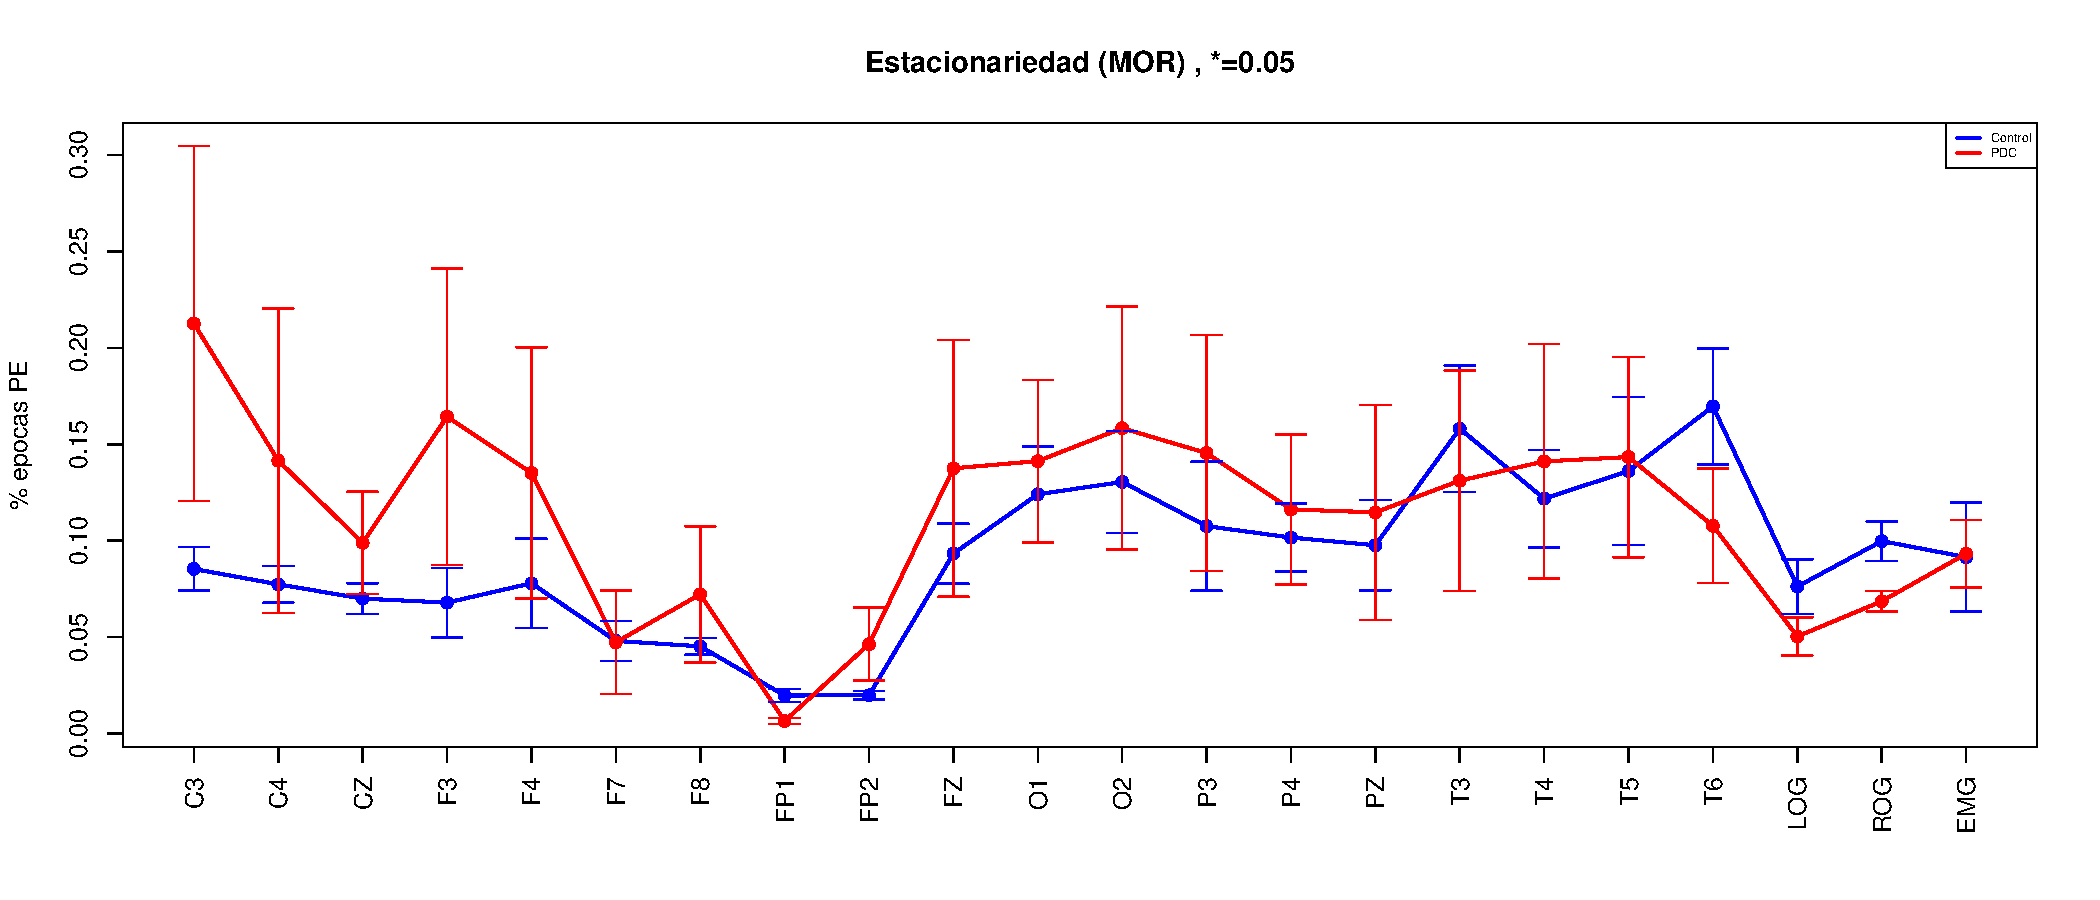
\includegraphics[width=0.95\linewidth]
{./new170424/Comparacion_gpos_MOR.pdf} 
}\\
\subfloat[Comparaci\'on entre \'epocas no-MOR (fases W y N)]{
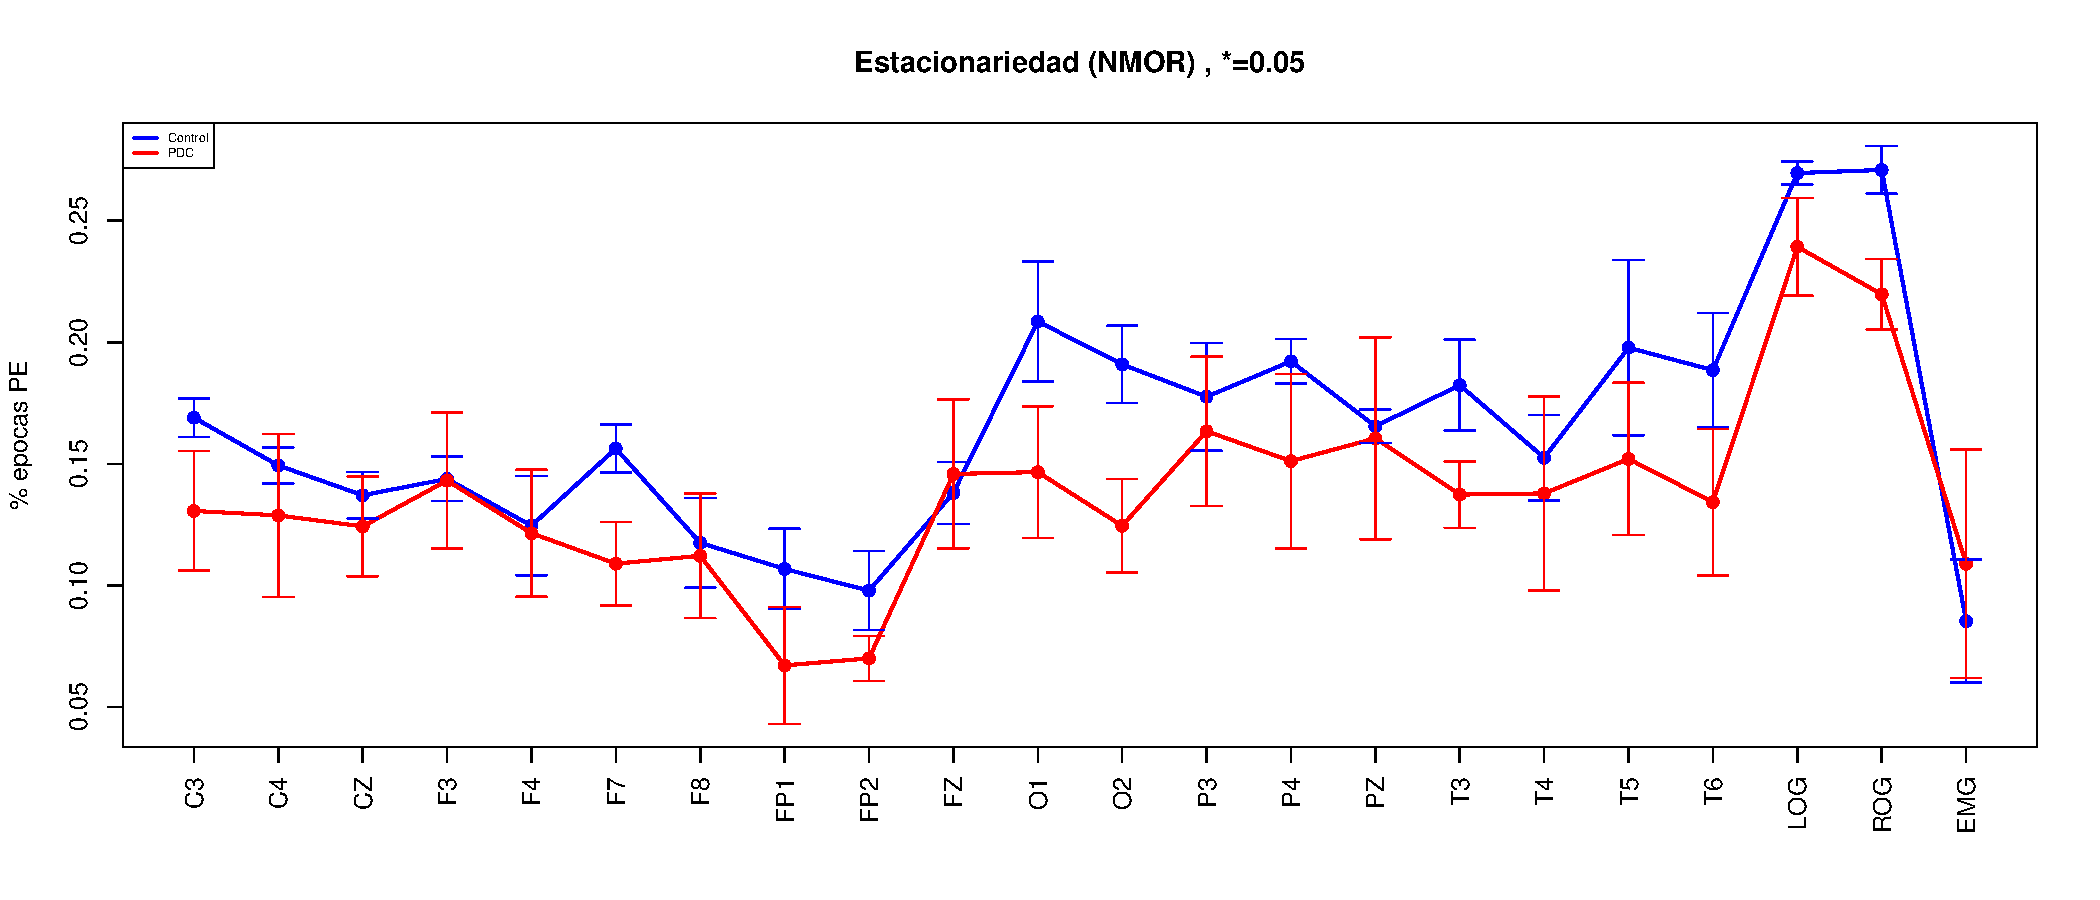
\includegraphics[width=0.95\linewidth]
{./new170424/Comparacion_gpos_NMOR.pdf} 
}\\
%\subfloat[Comparaci\'on entre el total de \'epocas registradas]{
%\includegraphics[width=0.95\linewidth]
%{./muypreeliminar170408/Comparacion_gpos_TOT.png} 
%}\\
\caption{Comparaci\'on sobre las proporciones de \'epocas PE entre los grupos, para diferentes
etapas de sue\~no. Se han graficado las proporciones de PE en todos los sujetos de ambos grupos,
as\'i como sus respectivos promedios, para cada etapa de sue\~no.}
\label{comparacion_graf}
\end{figure}

La comparaci\'on per se se llev\'o a cabo usando la prueba %no param\'etrica
%$t$ de Student y 
$U$ de Mann-Whitney\footnote{Implementada en R como la funci\'on \texttt{wilcox.test()}}.
%El primer test arroja diferencias significativas para los canales LOG, ROG y EMG, mientras que
%el segundo indica que no hay diferencias significativas. 
No se encontraron diferencias significativas para ninguno de los canales.

%Debido a que los canales
%donde se hallaron diferencias significativas no corresponden a registros de actividad
%cerebral, se considera que \textbf{esta caracter\'istica no proporciona evidencias
%suficientes sobre diferencias significativas entre adultos mayores con y sin PDC diagnosticado}.
%Este resultado es clave en el desarrollo de este trabajo.

Una tercera prueba efectuada sobre los datos fue una comparaci\'on para la proporci\'on de \'epocas
PE en cada canal, para revisar diferencias grupales entre sue\~no MOR y NMOR.
Esta prueba tiene una interpretaci\'on m\'as bien complicada, aunque su motivaci\'on es clara:
una vez hecha la comparaci\'on individial de las proporciones de PE al 
''transitar'' los sujetos entre etapas de sue\~no, y viendo que 
no hay diferencias claras entre grupos, cabe preguntarse si conviene considerar a los grupos 
como unidades.
Se encuentra que hay diferencias significativas ($\alpha<.1$) para el grupo normal
en los canales C3, C4, F7, F8, FP1, FP2, O2, P4, LOG, ROG; en el grupo PDC no se encontr\'o
ninguna diferencia.
Las diferencias encontradas pueden ser relevantes fisiol\'ogicamente, ya que 
abarcan gran parte de los l\'obulos frontal y parietal, y una regi\'on occipital-parietal derecha.
Se resta importancia a las diferencias halladas en LOG y ROG, ya que en el grupo PDC puede
aceptarse esta diferencia ''con no mucha probabilidad'' ($\alpha<.15$) y porque se esperaba
esta diferencia t\'ipica del sue\~no MOR

\begin{figure}
\centering
\subfloat[Comparaci\'on para el grupo control]{
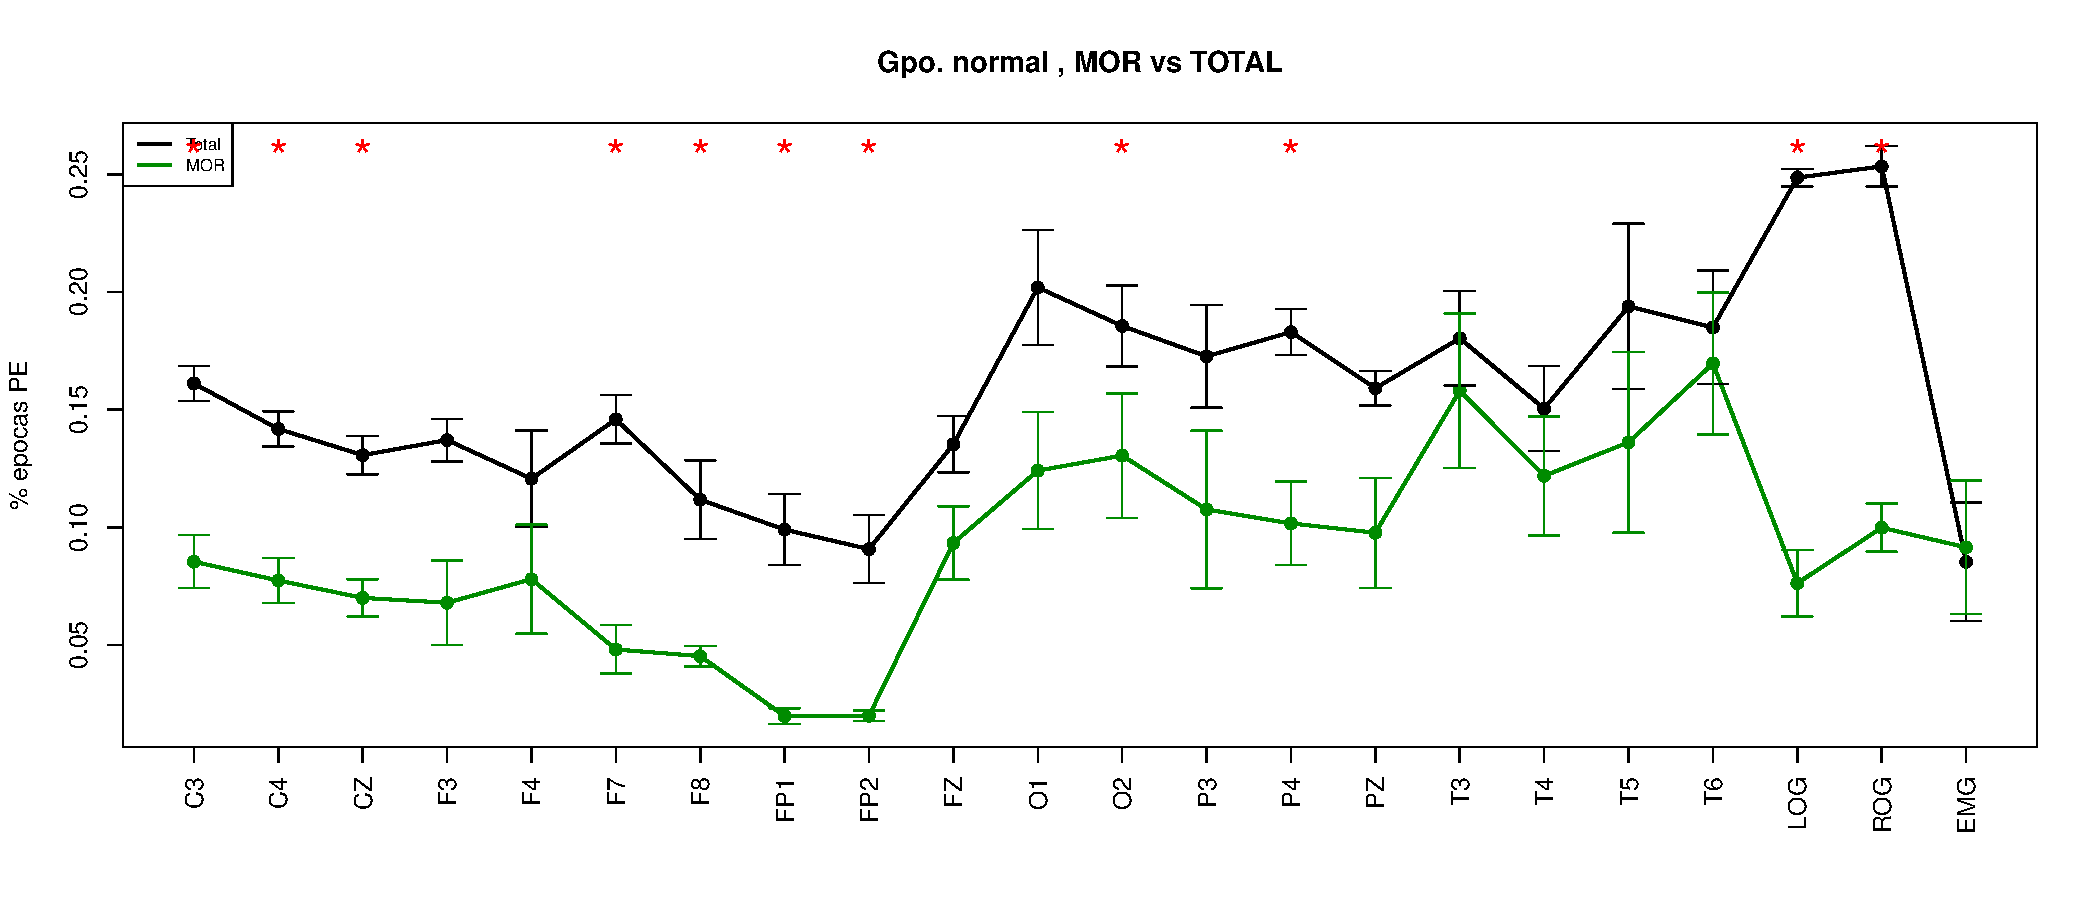
\includegraphics[width=0.95\linewidth]
{./new170424/comp_etapas_gpos_NORMALMOR_vs_TOTAL.pdf} 
}\\
\subfloat[Comparaci\'on para el grupo PDC]{
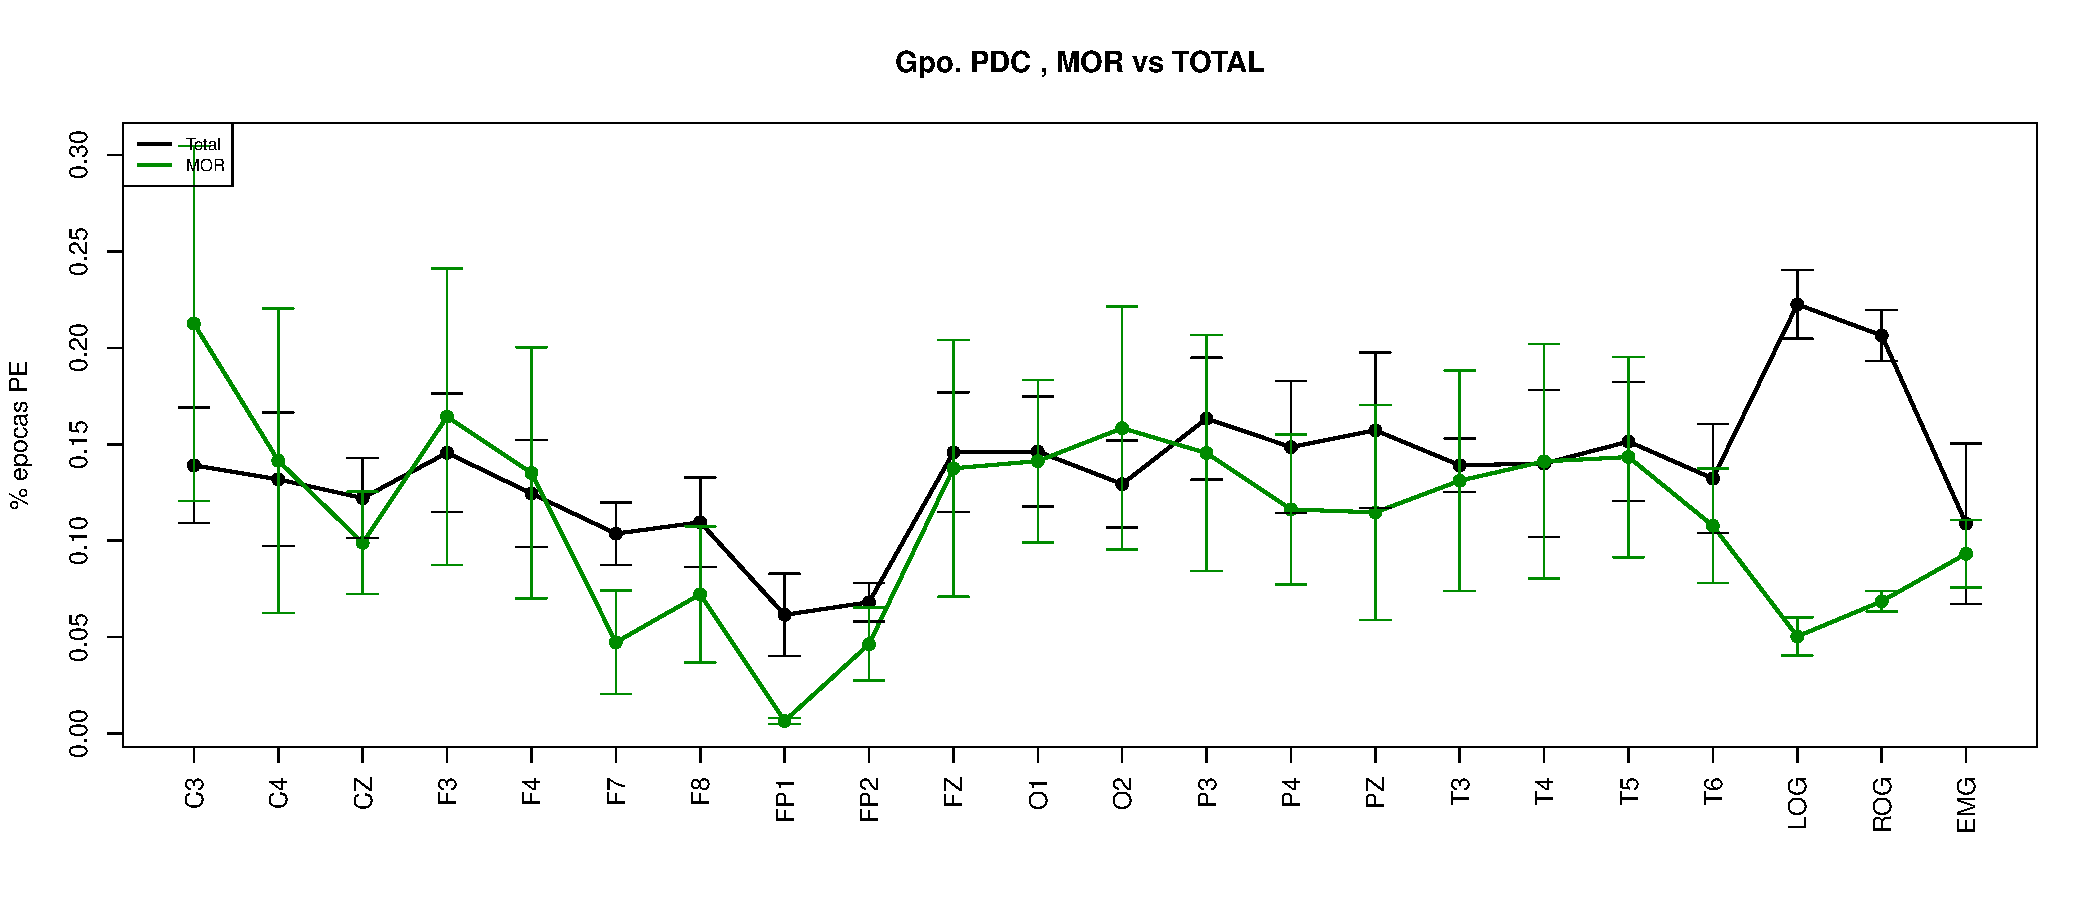
\includegraphics[width=0.95\linewidth]
{./new170424/comp_etapas_gpos_PDCMOR_vs_TOTAL.pdf} 
}\\
\subfloat[Comparaci\'on de los p-valores para aceptar diferencias]{
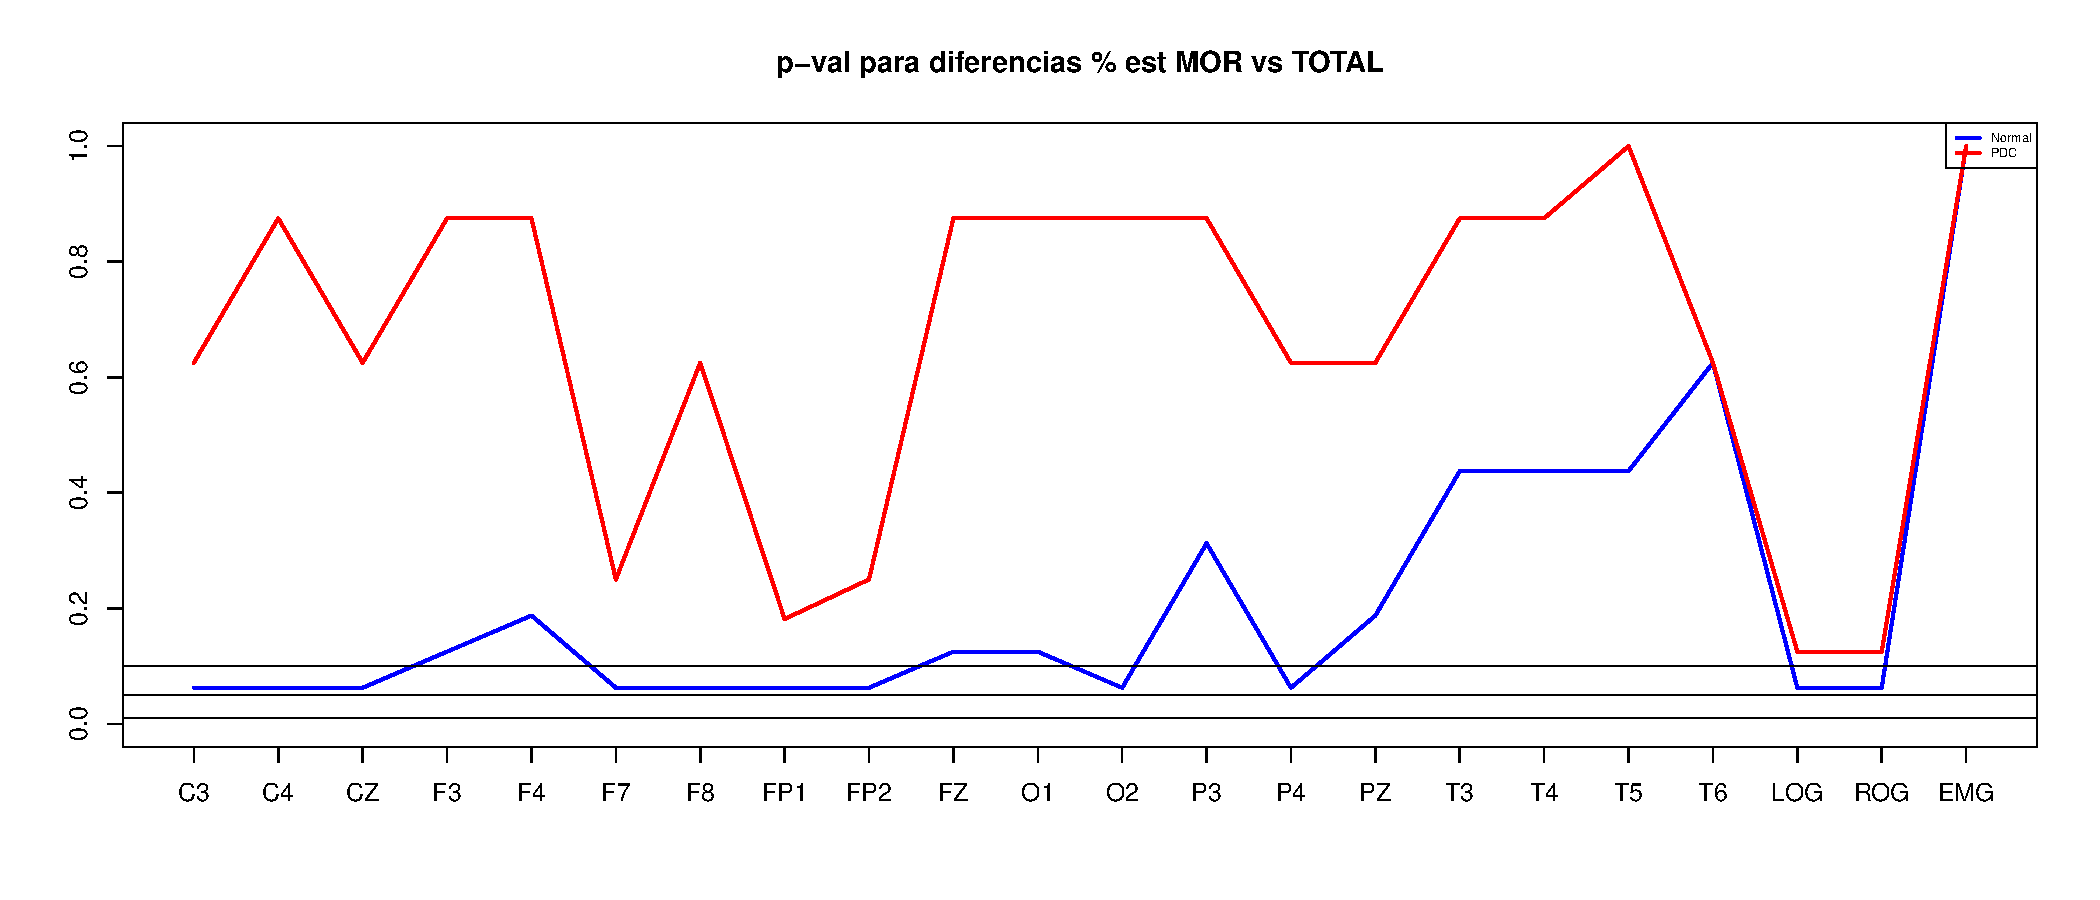
\includegraphics[width=0.95\linewidth]
{./new170424/Comparacion_pvals_gpos_MOR_vs_TOTAL.pdf} 
}\\
\caption{Comparaci\'on sobre las proporciones de \'epocas PE entre las etapas de sue\~no, 
para ambos grupos por separado. 
Se han graficado las proporciones de PE en todos los sujetos de cada grupo,
para todo el sue\~no y la etapa MOR.}
\label{comparacion_verde}
\end{figure}

\begin{figure}
\centering
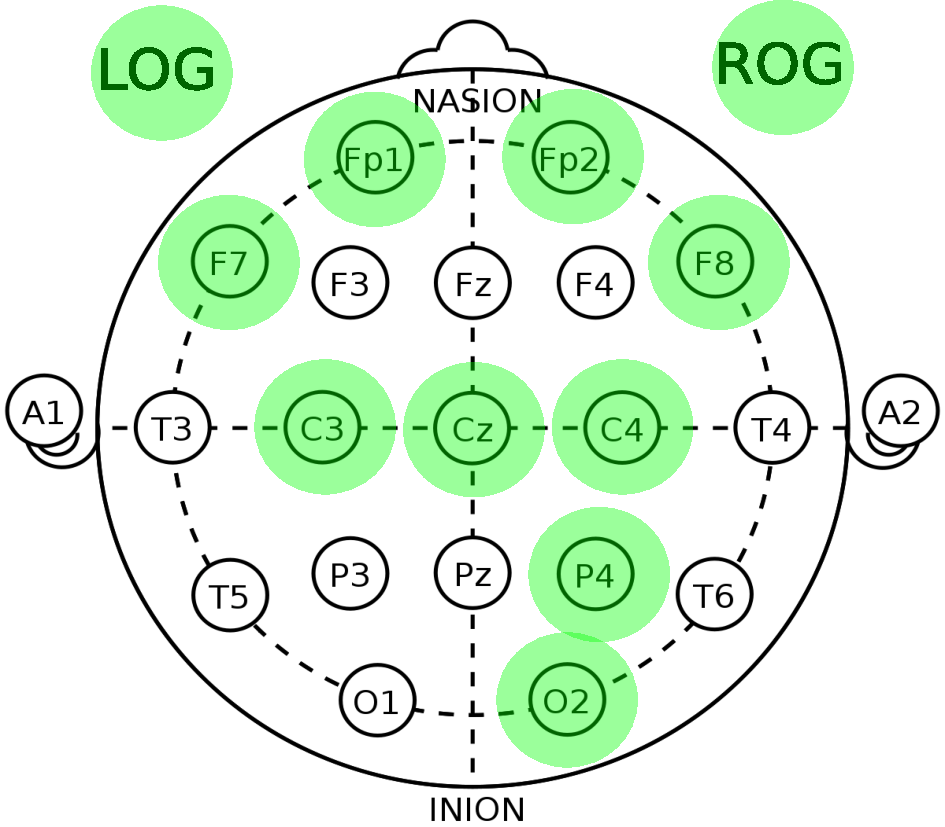
\includegraphics[width=0.65\linewidth]
{cabecita.pdf} 
\caption{Representaci\'on esquem\'atica de los sitios donde se encontraron diferencias significaticas}
\label{cabecita}
\end{figure}


Un \'ultimo an\'alisis que ser\'a reportado, es 
respecto a
una forma particular en que se han graficado los
datos obtenidos y que parece contener informaci\'on relevante.
Para esta disposici\'on gr\'afica, se colocaron en l\'inea horizontal 
''cuadros'' blanco y negros por cada
\'epoca analizada seg\'un haya sido clasificada usando el test PSR 
(blanco para PE, negro para no-estacionario)
Puede verse en la figura \ref{ejemplo_graf} un ejemplo de esta disposici\'on gr\'afica, mientras
que el resto de estos gr\'aficos se incluye como anexo.

\begin{figure}
\includegraphics[width=\textwidth]%{MJNNVIGILOS_127_mor127_tot1032_esttotal.pdf} 
{./g170413/MJNNVIGILOS_est.png}
\caption{Disposici\'on gr\'afica para los resultados del test PSR en el sujeto MJH., 
%para 1032 \'epocas de sue\~no y 22 canales. 
En el eje horizontal se muestra el tiempo desde el inicio de registro, en el eje vertical se 
muestra el nombre del canal. 
Se han resaltado con color verde las \'epocas clasificadas como de 
sue\~no MOR.
%, que son 127.
%Para este gr\'afico las \'epocas PE se clasificaron si la hip\'otesis de estacionaeriedad
%se pod\'ia rechazar la hip\'otesis de estacionariedad con en p-valor de 0.05
%seg\'un el test PSR.
}
\label{ejemplo_graf}
\end{figure}

Una debilidad 
a considerar sobre estos gr\'aficos
%importante de los gr\'aficos as\'i obtenidos 
es que, si bien hay patrones 
visuales en el tiempo,
deben ser definidos formalmente y cuantizados antes de poder ser
estudiados de manera efectiva; esta tarea ha sido poco fruct\'ifera 
y no ha aportado datos relevantes en cuanto a los objetivos planteados en un principio,
de modo que se ha exclu\'ido del cuepro principal de este trabajo.
%
% \'estos no se pueden cuantificar de una manera obvia y se dificulta la
%comparaci\'on entre sujetos, raz\'on por la cual se omiti\'o del cuerpo principal del trabajo. 
%%Se han inclu\'ido estos resultados porque sus caracter\'isticas 
%%sugieren una posible utilizaci\'on para otros fines --en alg\'un trabajo futuro.

Al ''calcular'' estos gr\'aficos para cada sujeto,
%Dentro de un mismo sujeto, 
aparecen diferencias cualitativas visibles
entre el sue\~no MOR y el resto del sue\~no nocturno; en la figura
\ref{patroncito} se muestra este patr\'on visual propuesto que,
%que vagamente est\'a caracterizado que, 
se observa, siempre contiene al sue\~no MOR si \'este no es fragmentado.
Se propone la siguiente caracterizaci\'on
para el patr\'on:
\begin{itemize}
\item Un ''bloque'' con muy pocas \'epocas PE, seguido por un bloque abundante en
\'epocas PE
\item Un bloque con una cantidad ''media'' de \'epocas PE en casi todos los canales,
excepto en LOG y ROG donde pr\'acticamente est\'an ausentes
\item Un bloque con muchas \'epocas PE en LOG y ROG, que interrumpe el bloque anterior
\end{itemize}
%Se observa que el segundo bloque siempre contiene al sue\~no MOR, si este no es fragmentado.
El tercer bloque, casi carente de \'epocas PE en los cnales LOG y ROG, parece contener
al sue\~no MOR si bien no es muy espec\'ifico. En un anexo se incluyen
todos los gr\'aficos obtenidos de esta forma.

\begin{figure}
\includegraphics[width=\textwidth]
%{./complementario170409/patrones_MJH.png}
{./graphs170427/zoom_MFGR.pdf}
\caption{Se han resaltado con color azul 
los patrones gr\'aficos 
cualitativos propuestos.}
\label{patroncito}
\end{figure}

Conviene mencionar que el origen de esta representaci\'on gr\'afica es un intento preeliminar de
fragmentar los an\'alsis de sue\~no MOR en grupos de \'epocas consecutivas en sue\~no MOR ya que,
en general, eesta etapa aparece fragmetnada durante el sue\~no nocturno \cite{CarrilloMora};
en otras palabras, existe una vaga motivaci\'on fisiol\'ogica para investigar estos patrones.
%La hip\'otesis de que se podr\'ian definir diferencias que involucraran la componente espacial,
%sin embargo, se vio opacada por la dificultad de definir formalmente tales diferencias a modo
%que pudieran compararse entre sujetos.
%Una sugerencia recibida consiste en seguir explorando estos patrones en el tiempo, pero quiz\'a
%no con la intenci\'on de detectar deterioro cognitivo sino como apoyo para la identificaci\'on de
%diferentes etapas de sue\~no.

Las hip\'otesis vertidas aqu\'i respecto a los patrones se mantendr\'an como comentarios
al cierre de este trabajo,
o como posible motivaci\'on para un trabajo futuro;
debido a que el hallazgo puede clasificarse como incidental, era menester mencionarlo.

%%%%%%%%%%%%%%%%%%%%%%%%%%%%%%%%%%%%%%%%%%%%%%%%%%%%%%%%%%%%%%%%%%%%%%%%%%%%%%%%%%%%%%%%%%%%%%%%%%%
%%%%%%%%%%%%%%%%%%%%%%%%%%%%%%%%%%%%%%%%%%%%%%%%%%%%%%%%%%%%%%%%%%%%%%%%%%%%%%%%%%%%%%%%%%%%%%%%%%%